%=================================================================
\section{Introduction}\label{sec-intro}
\subsection{Describe the Problem}
\smallskip
This is a problem with time-series prediction. Many information are given about daily sales data.The raw dataset contains train set with 2935849 samples and 214200 unlabeled samples as test set. Through the train data, predict total sales for every product and store in the next month.
\subsection{Interpret the Data}
\smallskip
Here's the data in the dataset.\\
\bigskip
\centerline{\normalsize{Table 1:Data}}
\begin{tabular}{cp{4cm}p{4cm}}
	\hline
	Name&Description&Attribute\\
	\hline
	sales\_train.csv& Training set(data from January 2013 to October 2015)&date,date_block_num, shop_id,item_id, item_price,item_cnt_day\\
	test.csv& Test set(Predict sale in November 2015) & ID,shop_id,item_id\\
	items.csv& Supplementary information of products &item_name, item_id, item_category_id\\
	shops.csv& Supplementary information of shops & shops_name,  shops_id\\
	item_categories.csv& Supplementary information of item categories & item_categories_name, item_categories_id\\
	sample_submission.csv& Format of submission & ID,item_cnt_month\\
	\hline
\end{tabular}
\subsection{Evaluation Criteria}
Before experiment, determine the evaluation methods to assess the model performance is very important, usually it has the RMSE methods to evaluate.
\section{Data Processing} \label{sec-preliminaries}	
\subsection{Missing Value and NaN Value} There are no missing value and none value.
	\begin{figure}[htb]
	\centering
	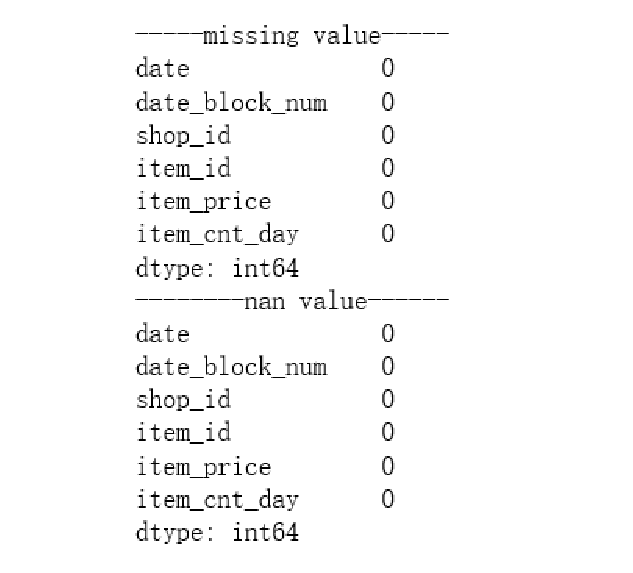
\includegraphics[width=8cm, height=6cm]{figures/miss.eps}\\
	\caption{Missing Value and NaN Value
	}\label{straddltimeScale}
\end{figure}
\subsection{Outliers and Duplicate Data} Filter duplicate data, outliers and data with price less than zero.
\begin{figure}[htb]
	\centering
	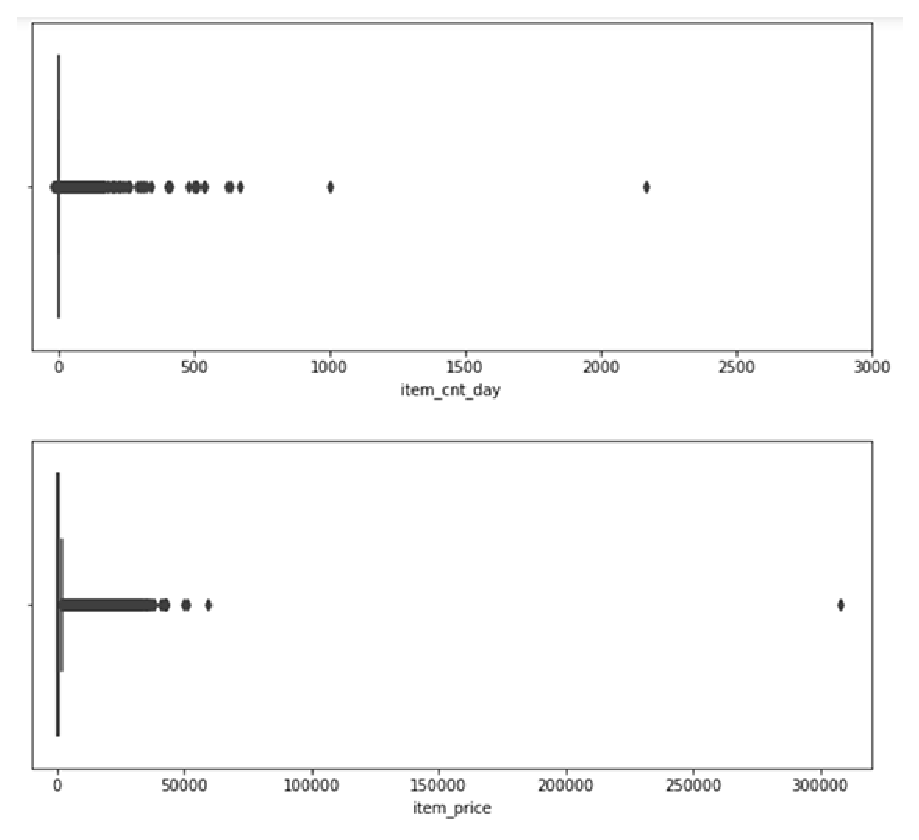
\includegraphics[width=10cm, height=8cm]{figures/outliers.eps}
	\caption{Outliers Data
	}\label{straddltimeScale}
\end{figure}
\subsection{Sales Analysis}	Figure3 shows that total sales every month are decreased over time. This reason probably is shops and items are decreased. By analyzing the data, there are many discontinued items in figure4 and these shops are closed:closed shops:0,1,8,11,13,17,23,27,29,30,32,33,40,43,51,54.
	\begin{figure}[htb]
	\centering
	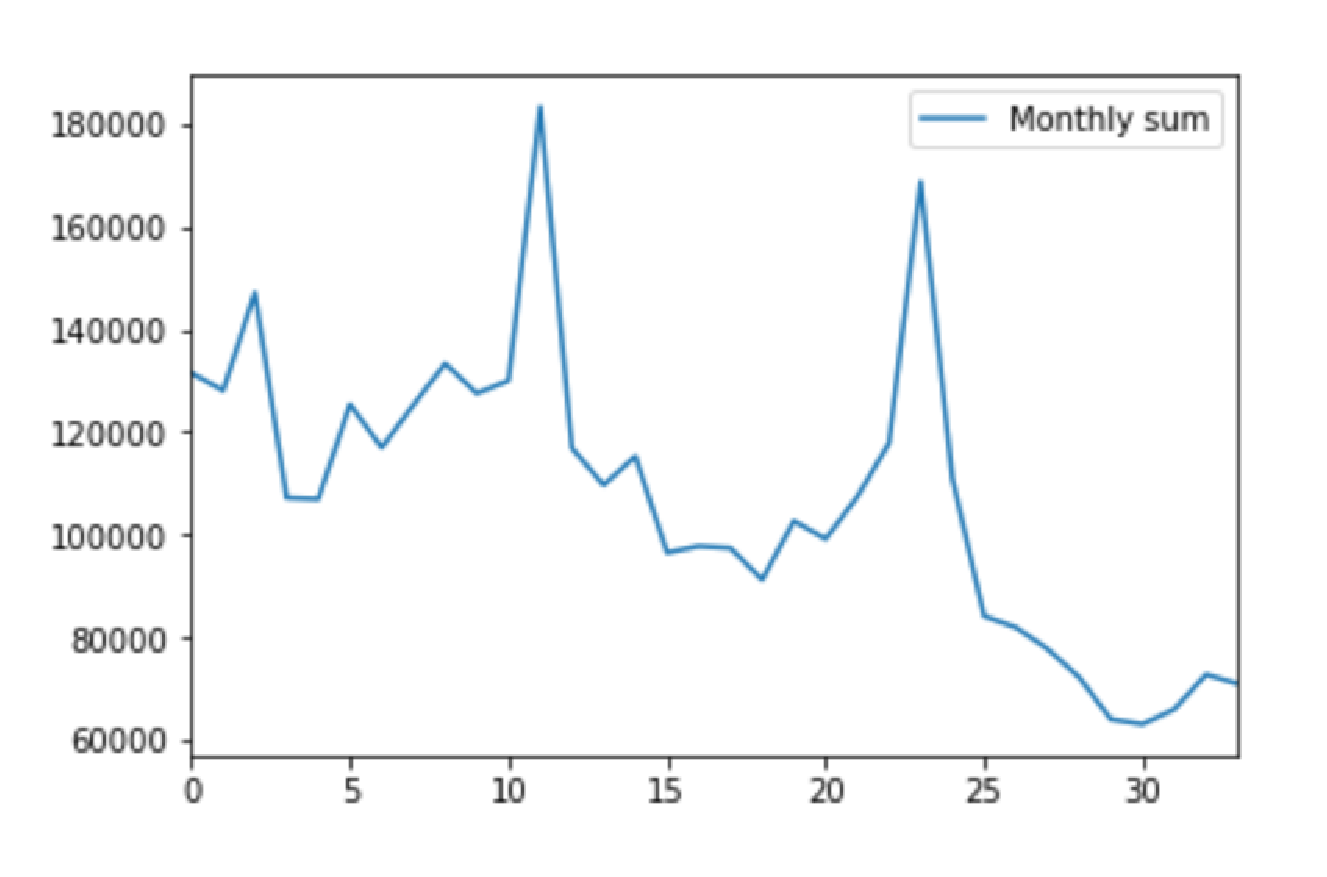
\includegraphics[width=10cm, height=6cm]{figures/sum.eps}
	\caption{Total Sales Over Time
	}\label{straddltimeScale}
\end{figure}
\begin{figure}[htb]
	\centering
	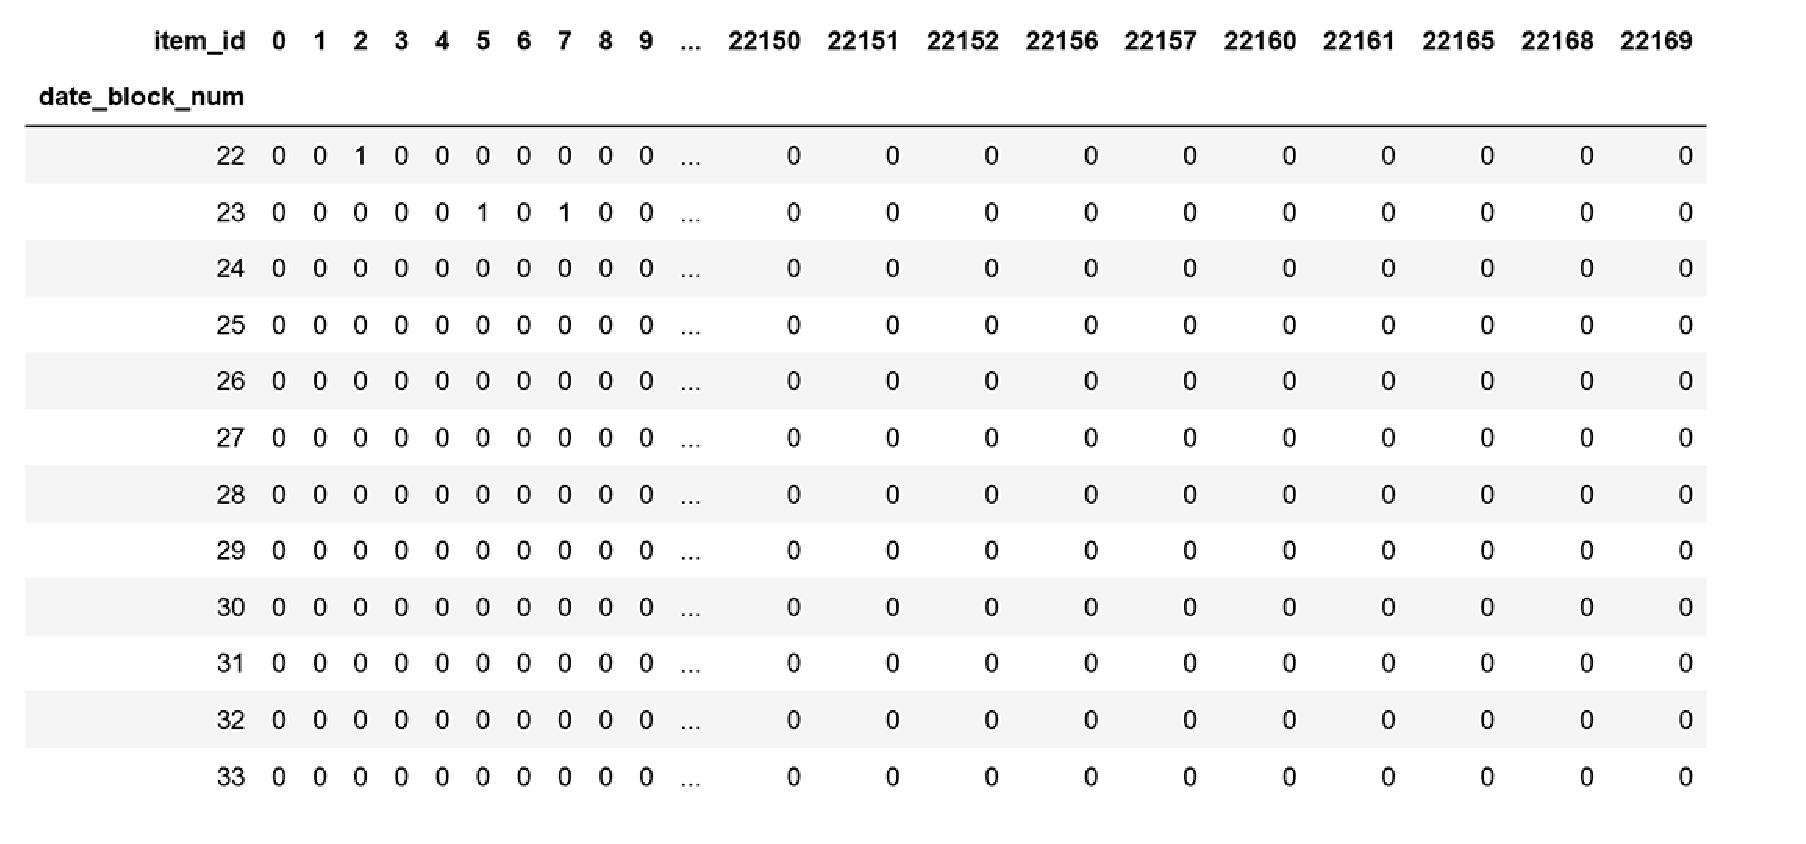
\includegraphics[width=12cm, height=6cm]{figures/stopitems.eps}
	\caption{Discontinued Products
	}\label{straddltimeScale}
\end{figure}
\section{Feature Selection} \label{sec-method}	
This report simply counts monthly sales of every items, and choose each item every month sales and item categories as feature, final matrix is figure5.
\begin{figure}[htb]
	\centering
	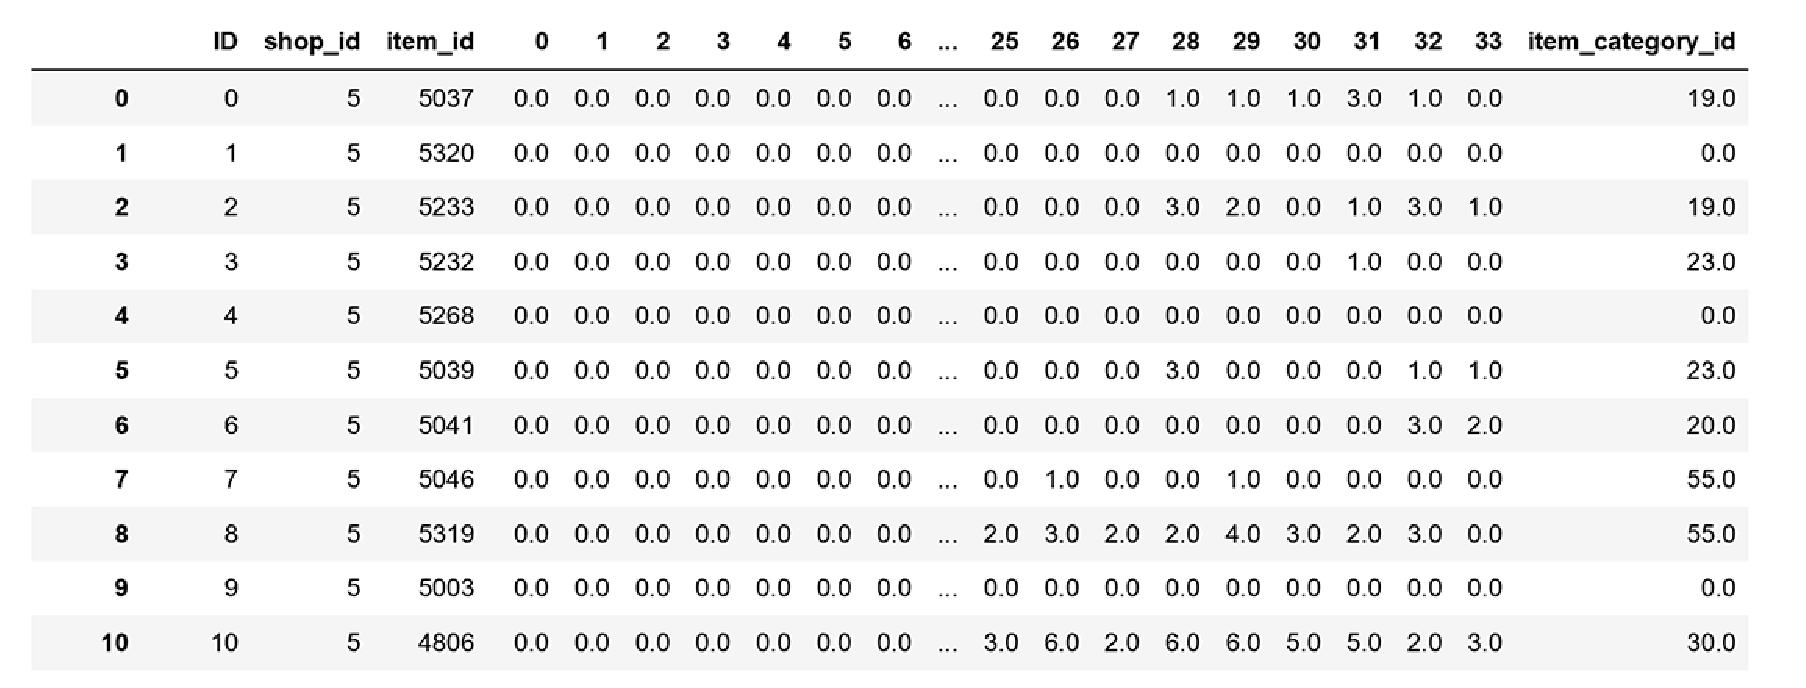
\includegraphics[width=12cm, height=6cm]{figures/feature1.eps}
	\caption{Discontinued Products
	}\label{straddltimeScale}
\end{figure}
\section{Experiment and Analysis} \label{sec-experiment}
Using xgboost to predict the sales. And in the final database, change zero to closed shops and discontinued items.\\
XGBoost is to establish K regression trees so that the predicted value of the tree group is as close as possible to the true value (accuracy) and has the greatest generalization ability. From a mathematical point of view, this is a functional optimization, multi-target.
The final score is 1.04885 and get the middle rank.
\begin{figure}[htb]
	\centering
	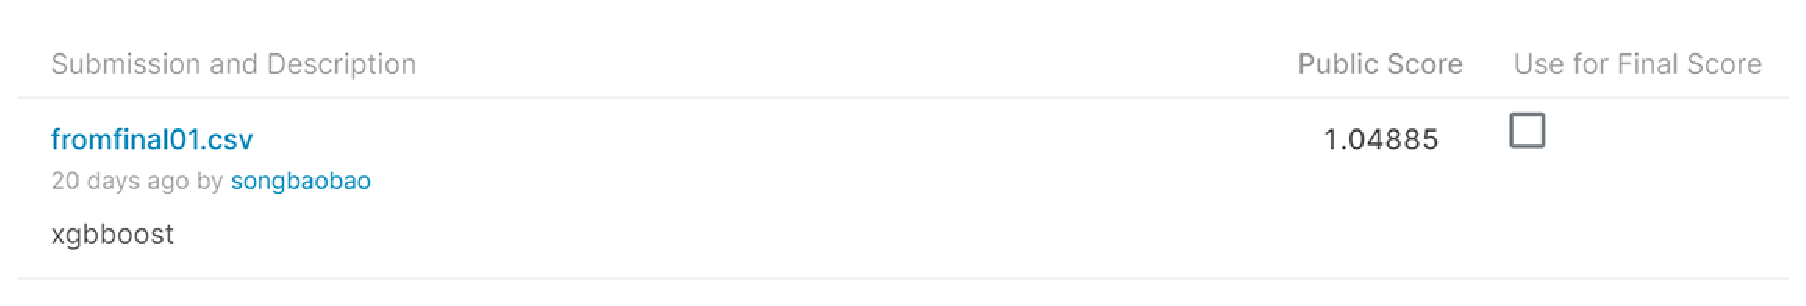
\includegraphics[width=12cm, height=2cm]{figures/rmse1.eps}
	\caption{Discontinued Products
	}\label{straddltimeScale}
\end{figure}
\section{Conclusions} \label{sec-conclusions}
\begin{itemize}
	\item the features are little.
	\item The model is not trained.
\end{itemize}

\section*{Acknowledgment}

\lipsum[1]


The authors would like to thank \ldots

